\documentclass{ximera}

\input{../preamble}
\author{Elizabeth Campolongo}
\license{Creative Commons Attribution-ShareAlike 4.0 International License}
\acknowledgement{https://activecalculus.org/prelude/sec-trig-inverse.htmll}
\acknowledgement{https://www.stitz-zeager.com/szprecalculus07042013.pdf}

\title{Other Inverse Trig Functions}

\begin{document}
\begin{abstract}
  
\end{abstract}
\maketitle


%\typeout{************************************************}
%\typeout{Motivating Questions}
%\typeout{************************************************}

\begin{motivatingQuestions}\begin{itemize}
%Often start a section. 
\item For the restricted sine and tangent functions, how do we define the corresponding arcsine and arctangent functions?
\item What are the key properties of arcsine and arctangent?
\end{itemize}\end{motivatingQuestions}


%\typeout{************************************************}
%\typeout{Introduction}
%\typeout{************************************************}



%\typeout{************************************************}
%\typeout{section}
%\typeout{************************************************}

\section{Introduction}
In the last section we defined {\it arccosine}, the inverse for cosine restricted to a single period. In this section we will explore the definition of similar inverse functions on restricted domains of sine and tangent. 

As we recalled last time,
\begin{itemize}
\item
A function $f$ has an inverse function if and only if there exists a function $g$ that undoes the work of $f$: that is, there is some function $g$, the inverse of $f$, for which $g(f(x)) = x$ for each $x$ in the domain of $f$, and $f(g(y)) = y$ for each $y$ in the range of $f$. 
%
\item A function $f$ has an inverse function if and only if the graph of $f$ passes the {\it Horizontal Line Test}.
%
\item When $f$ has an inverse, we know that ``$y = f(t)$'' and ``$t = f^{-1}(y)$'' are two different perspectives on the same statement.
\end{itemize}
%
\par
As with the cosine function, the trigonometric functions $f(t) = \sin(t)$ and $h(t) = \tan(t)$ are periodic, so they fail the horizontal line test. Hence, considering these functions on their full domains, neither has an inverse function. At the same time, it is reasonable to think about changing perspective and viewing angles as outputs in certain restricted settings, as we did with cosine. 


\section{The Arcsine Function}

We can develop an inverse function for a restricted version of the sine function in a similar way.  As with the cosine function, we need to choose an interval on which the sine function is always increasing or always decreasing in order to have the function pass the horizontal line test.  The standard choice is the domain $\Big[\!\!-\!\frac{\pi}{2}, \frac{\pi}{2}\Big]$ on which $f(t) = \sin(t)$ is increasing and attains all of the values in the range of the sine function.  Thus, we consider $f(t) = \sin(t)$ so that $f : \Big[\!-\frac{\pi}{2}, \frac{\pi}{2}\Big] \to \big[\!-1,1\big]$ and use this restricted function to define the corresponding arcsine function.%
\begin{definition}
Let $y = f(t) = \sin(t)$ be defined on the domain $\Big[\!\!-\!\frac{\pi}{2}, \frac{\pi}{2}\Big]$, and observe $f : \Big[\!-\frac{\pi}{2}, \frac{\pi}{2}\Big] \to \big[\!-1,1\big]$.  For any real number $y$ that satisfies $-1 \leq y \leq 1$, the \dfn{arcsine of $\mathbf{y}$}, denoted%
\begin{equation*}
\arcsin(y)
\end{equation*}
is the angle $t$ satisfying $-\frac{\pi}{2} \leq t \leq \frac{\pi}{2}$ such that $\sin(t) = y$.
%
Note that we use $t=\sin^{-1}(y)$ interchangeably with with $t = \arcsin(y)$. 
\end{definition}

\begin{problem}
The goal of this activity is to understand key properties of the arcsine function in a way similar to our discussion of the arccosine function in the previous section. We will use our deductive reasoning skills a la Sherlock Holmes to build off our discussion from the last section.%
\begin{enumerate}
\item
Using the definition of arcsine given above, what are the domain and range of the arcsine function? \\
\begin{itemize}
\item The domain of arcsine is $\answer{[-\frac{\pi}{2},\frac{\pi}{2}]}$.
%
\item The range of arcsine is $\answer{[-1,1]}$.
\end{itemize}
%
\item Determine the following values exactly: 
\begin{itemize}
\item $\arcsin(-1) = \answer{-\frac{\pi}{2}}$ 
%
\item $\arcsin\Big(\!\!-\frac{\sqrt{2}}{2}\Big) = \answer{-\frac{\pi}{4}}$
%
\item $\arcsin(0) = \answer{0}$
%
\item $\arcsin\Big(\frac{1}{2}\Big) = \answer{\frac{\pi}{6}}$
%
\item $\arcsin\Big(\frac{\sqrt{3}}{2}\Big) = \answer{\frac{\pi}{3}}$
\end{itemize}
%
\item
On the axes provided below, sketch a careful plot of the restricted sine function on the interval $\Big[\!\!-\!\frac{\pi}{2},\frac{\pi}{2}\Big]$ along with its corresponding inverse, the arcsine function.  Label at least three points on each curve so that each point on the sine graph corresponds to a point on the arcsine graph.  In addition, sketch the line $y = t$ to demonstrate how the graphs are reflections of one another across this line.
%
%
\item True or false: $\arcsin(\sin(5\pi)) = 5\pi$? $\wordChoice{\choice{\text{true}}\choice[correct]{\text{false}}}$ \\
Write a complete sentence to explain your reasoning.%
\end{enumerate}
\includegraphics[width=1\linewidth]{inverse-trig-blank-axes-arcsin.pdf}
\end{problem}

\begin{callout}{\bf Properties of the arcsine function.}%
\begin{itemize}
\item
The restricted sine function, $y = f(t) = \sin(t)$, is defined on the domain $\Big[\!\!-\!\frac{\pi}{2},\frac{\pi}{2}\Big]$ with range $[-1,1]$.  This function has an inverse function that we call the arcsine function, denoted $t = f^{-1}(y) = \arcsin(y)$.%
\item
The domain of $y = f^{-1}(t) = \arcsin(t)$ is $[-1,1]$ with range $\Big[\!-\!\frac{\pi}{2},\frac{\pi}{2}\Big]$.%
\item
The arcsine function is always increasing on its domain.%
\item
Below we have a plot of the restricted sine function (in light blue) and its corresponding inverse, the arcsine function (in dark blue).%
\end{itemize}
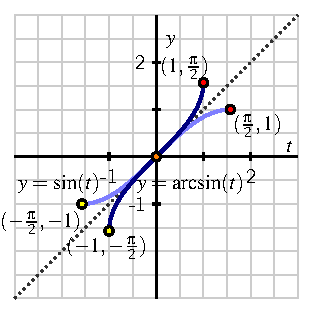
\includegraphics[width=1\linewidth]{inverse-trig-arcsin-graph.pdf}
\end{callout}

\section{Exploring Arcsine}

\begin{example}
Let's solve the following equations analytically, then we can consider the graph of arcsine.

\begin{enumerate}
\item $\sin\!\Big(\!\arcsin\!\Big(\!-\frac{\sqrt{2}}{2}\Big)\Big)$\\
\begin{explanation}
We start by finding $\arcsin\!\Big(\!\!-\!\frac{\sqrt{2}}{2}\Big)$. Remember that for $x$ in $[-1,1]$, $\arcsin(x)$ is the value $y$ in $\Big[-\frac{\pi}{2},\frac{\pi}{2}\Big]$ such that $\sin(y) = x$. 

Hence, $y$ is $-\frac{\pi}{4}$, and we now see that 
\begin{equation*}
\sin\!\Big(\!\arcsin\!\Big(\!\!-\!\frac{\sqrt{2}}{2}\Big)\Big) = \sin\Big(\!-\frac{\pi}{4}\Big) = -\frac{\sqrt{2}}{2}.
\end{equation*}

Now, if you're thinking, ``Hey, we didn't need that extra step!" Then you would be correct. But \textbf{\textit{why}} didn't we need that final step?

Let's recall how we defined arcsine. Since sine is a periodic function, it fails the horizontal line test. However, if we {\it restrict} sine to a portion of its domain on which it is only increasing, $\Big[-\frac{\pi}{2},\frac{\pi}{2}\Big]$, then we may define a function $f$ on this domain such that $f(x) = \sin(x)$ for $x$ in $\Big[-\frac{\pi}{2},\frac{\pi}{2}\Big]$. Arcsine then is defined as the inverse of this function $f$. Therefore, $f$ is the inverse of arcsine. 
Thus, in practice, sine is the inverse of arcsine. 

A word of caution: As was the case with arccosine and cosine, arcsine is only the inverse of restricted sine. We will illustrate this with the next example.
\end{explanation}


\item $\arcsin\!\Big(\sin\!\Big(\frac{5\pi}{4}\Big)\Big)$

\begin{explanation}
It may be tempting to take a look at this expression and conclude that the solution is $\frac{5\pi}{4}$ since arcsine is the inverse of sine. 

{\bf Hold those horses! }

Remember, we had to restrict the domain of sine in order to define an inverse function, which we called arcsine. Arcsine is the inverse of the {\it restricted} sine function, whose domain is $\Big[\!-\frac{\pi}{2},\frac{\pi}{2}\Big]$. $\frac{5\pi}{4}$ is larger than $\frac{\pi}{2}$, so it is not within the domain of this restricted sine function. 

Thus, we begin by simplifying $\sin\!\Big(\frac{5\pi}{4}\Big) = -\frac{\sqrt{2}}{2}$. 

Now, let's consider $\arcsin\!\Big(\!\!-\!\frac{\sqrt{2}}{2}\Big)$, recalling again the {\it range} of arcsine. We are looking for the value of $y$ in $\Big[\!-\frac{\pi}{2},\frac{\pi}{2}\Big]$ such that $\sin(y) =-\frac{\sqrt{2}}{2}$.

Hence, $y$ is $-\frac{\pi}{4}$, and we now see that 
\begin{equation*}
\arcsin\!\Big(\sin\!\Big(\frac{5\pi}{4}\Big)\Big) = \arcsin\!\Big(\!\!-\!\frac{\sqrt{2}}{2}\Big) = -\frac{\pi}{4}.
\end{equation*}

[graph for arcsine?]
%Now, let's look again at the graph of cosine. Here we highlight $g: [0,\pi] \rightarrow [0,\pi]$ defined by $y=g(x)=\cos(x)$, the restricted cosine function. We may use the symmetry of the graph of cosine to help find the appropriate values for arccosine.
%\begin{image}
%\includegraphics{inverse-trig-PA-cosine.pdf}
%\end{image}

\end{explanation}

%=-\frac{\pi}{4}

\item $\arcsin(2x) = \frac{\pi}{3}$\\
\begin{explanation}
First, we observe that $\frac{\pi}{3}$ is in the range of arcsine, so there should be a solution. We will now use the fact that sine is the inverse of arcsine to reduce this to a linear equation.
\begin{align*}
\arcsin(2x) &= \frac{\pi}{3}\\
\sin(\arcsin(2x)) &= \sin(\frac{\pi}{3}) \\
\end{align*}
Thus, we have
$$2x = \frac{\sqrt{3}}{2},$$
which is equivalent to $x = \frac{\sqrt{3}}{4}$.

[Insert graph here?]
\end{explanation}
\end{enumerate}
\end{example}

\section{The Arctangent Function}
Finally, we develop an inverse function for a restricted version of the tangent function.  We choose the domain $\Big(\!-\frac{\pi}{2}, \frac{\pi}{2}\Big)$ on which $h(t) = \tan(t)$ is increasing and attains all of the values in the range of the tangent function.%
\begin{definition}
Let $y = h(t) = \tan(t)$ be defined on the domain $\Big(\!-\frac{\pi}{2}, \frac{\pi}{2}\Big)$, and observe $h : \Big(\!-\frac{\pi}{2}, \frac{\pi}{2}\Big) \to \big(-\infty,\infty\big)$.  For any real number $y$, the \dfn{arctangent of $\mathbf{y}$}, denoted%
\begin{equation*}
\arctan(y)
\end{equation*}
is the angle $t$ satisfying $-\frac{\pi}{2} < t <  \frac{\pi}{2}$ such that $\tan(t) = y$.
%
Note that we use $t=\tan^{-1}(y)$ interchangeably with with $t = \arctan(y)$. 
\end{definition}

\begin{problem}
Let us once again channel our inner Sherlock Holmes to understand key properties of the arctangent function.%
\par
\begin{enumerate}
\item Using the definition given above, what are the domain and range of the arctangent function?
%
\begin{itemize}
\item The domain of arctangent is $\answer{(-\frac{\pi}{2}, \frac{\pi}{2})}$.
%
\item The range of arctangent is $\answer{(-\infty,\infty)}$.
\end{itemize}
%
\item Determine the following values exactly: 
\begin{itemize}
\item $\arctan(-\sqrt{3}) = \answer{\frac{\pi}{3}}$
%
\item $\arctan(-1) = \answer{-\frac{\pi}{4}}$
%
\item $\arctan(0) = \answer{0}$
%
\item $\arctan\!\Big(\frac{1}{\sqrt{3}}\Big) = \answer{\frac{\pi}{6}}$.
\end{itemize}
%
\item The restricted tangent function on the interval $\Big(\!-\frac{\pi}{2}, \frac{\pi}{2}\Big)$ is plotted below. On the same axes, sketch its corresponding inverse function (arctangent).  Label at least three points on each curve so that each point on the tangent graph corresponds to a point on the arctangent graph. In addition, sketch the line $y = t$ to demonstrate how the graphs are reflections of one another across this line.%
%
\item Complete the following sentence:  ``as $t$ increases without bound, $\arctan(t)$ $\ldots$'' $\wordChoice{\choice{\text{increases without bound}}\choice{\text{decreases without bound}}\choice[correct]{\text{increases toward } \frac{\pi}{2}}\choice{\text{decreases toward } -\frac{\pi}{2}}}$%
\end{enumerate}
\includegraphics[width=1\linewidth]{inverse-tan-graph.pdf}
\end{problem}

\begin{callout}{\bf Properties of the arctangent function.}%
\begin{itemize}
\item
The restricted tangent function, $y = h(t) = \tan(t)$, is defined on the domain $\Big(\!\!-\frac{\pi}{2}, \frac{\pi}{2}\Big)$ with range $(-\infty,\infty)$.  This function has an inverse function that we call the arctangent function, denoted $t = h^{-1}(y) = \arctan(y)$.%
\item
The domain of $y = h^{-1}(t) = \arctan(t)$ is $(-\infty,\infty)$ with range $\Big(\!\!-\frac{\pi}{2}, \frac{\pi}{2}\Big)$.%
\item
The arctangent function is always increasing on its domain.%
\item
Below we have a plot of the restricted tangent function (in light blue) and its corresponding inverse, the arctangent function (in dark blue).%
\end{itemize}
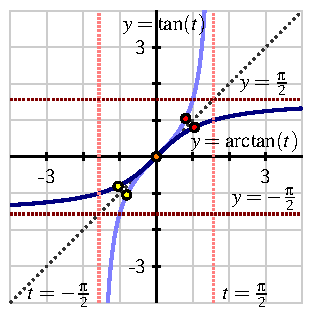
\includegraphics[width=1\linewidth]{inverse-trig-arctan-graph.pdf}
\end{callout}

\section{Exploring Arctangent}

\begin{example}
Let's solve the following equations analytically, then we can consider the graph of arctangent.	
\begin{enumerate}
\item

\item $\tan(\arctan(-\sqrt{3}))$\\
\begin{explanation}
We start by finding $\arctan(-\sqrt{3})$. Remember that for $x$ in $(-\infty,\infty)$, $\arctan(x)$ is the value $y$ in $\Big(\!-\frac{\pi}{2},\frac{\pi}{2}\Big)$ such that $\tan(y) = x$. 

Hence, $y$ is $-\frac{\pi}{3}$, and we now see that 
\begin{equation*}
\tan(\arctan(-\sqrt{3})) = \tan\Big(\!-\frac{\pi}{3}\Big) = -\sqrt{3}.
\end{equation*}

Now, I know you're thinking, ``Hey, why do you keep making us do an extra step?" It's because it is imperative that you \textbf{\textit{consider the range}} of the arc trig functions. These are considerations you will also need to make when we start combining different trig functions with the inverses of others (say sine of arctangent of a value).

Let's recall how we defined arctangent. Since tangent is a periodic function, it fails the horizontal line test. However, if we {\it restrict} tangent to a single period (note tangent only increasing), $\Big(\!-\frac{\pi}{2},\frac{\pi}{2}\Big)$, then we may define a function $h$ on this domain such that $h(x) = \tan(x)$ for $x$ in $\Big(\!-\frac{\pi}{2},\frac{\pi}{2}\Big)$. Arctangent then is defined as the inverse of this function $h$. Therefore, $h$ is the inverse of arctangent. 
Thus, in practice, tangent is the inverse of arctangent. 

A word of caution: As was the case with the previous two trig functions and their respective inverses, arctangent is only the inverse of restricted tangent. We will illustrate this with the next example.
\end{explanation}

%=-\sqrt{3}

\item $\arctan\!\Big(\!\tan\!\Big(\frac{5\pi}{3}\Big)\Big)$

\begin{explanation}
It may be tempting to take a look at this expression and conclude that the solution is $\frac{5\pi}{3}$ since arctangent is the inverse of tangent. 

{\bf But, wait! }

Remember, we had to restrict the domain of tangent in order to define an inverse function, which we called arctangent. Arctangent is the inverse of the {\it restricted} tangent function, whose domain is $\Big(\!-\frac{\pi}{2},\frac{\pi}{2}\Big)$. $\frac{5\pi}{3}$ is larger than $\frac{\pi}{2}$, so it is not within the domain of this restricted tangent function. 

Thus, we begin by simplifying $\tan\!\Big(\frac{5\pi}{3}\Big) = -\sqrt{3}$. 

Now, let's consider $\arctan(-\sqrt{3})$, recalling again the {\it range} of arctangent. We are looking for the value of $y$ in $\Big(\!-\frac{\pi}{2},\frac{\pi}{2}\Big)$ such that $\tan(y) =-\sqrt{3}$.

Hence, $y$ is $-\frac{\pi}{3}$, and we now see that 
\begin{equation*}
\arctan\!\Big(\!\tan\!\Big(\frac{5\pi}{3}\Big)\Big) = \arctan(-\sqrt{3}) = -\frac{\pi}{3}.
\end{equation*}

[graph for arctangent?]
%Now, let's look again at the graph of cosine. Here we highlight $g: [0,\pi] \rightarrow [0,\pi]$ defined by $y=g(x)=\cos(x)$, the restricted cosine function. We may use the symmetry of the graph of cosine to help find the appropriate values for arccosine.
%\begin{image}
%\includegraphics{inverse-trig-PA-cosine.pdf}
%\end{image}

\end{explanation}

% = -\frac{\pi}{3}$

\item $4\arctan^2(x) - 3\pi \arctan(x) - \pi^2 = 0$\\
\begin{explanation}
	We will treat this like a quadratic equation to begin, as we did in Section 10-3 Some Applications of Trig Functions. 

Let $y = \arctan(x)$, then we have a standard quadratic equation: $4y^2- 3\pi y - \pi^2=0$. Factoring, we see that this is equivalent to 
$$(4y +\pi)(y-\pi)=0.$$
%
This has two solutions: $y = -\frac{\pi}{4}$ and $y=\pi$. In other words, we now simply solve (a) $\arctan(x) = -\frac{\pi}{4}$ and (b) $\arctan(x) = \pi$. $\pi$ is not in the range of arctangent, so (b) does not have a solution. Hence, this cannot be a solution to our equation, and we must look at (a). $-\frac{\pi}{4}$ is in the range of arctangent, so the solution to (a) will be a solution to our original equation.

Since tangent is the inverse to arctangent, the equation (a) is equivalent to $$\tan(\arctan(x))=\tan\!\Big(\!-\frac{\pi}{4}\Big),$$
which is further equivalent to $x=-1$
\end{explanation}
\end{enumerate}
\end{example}



\begin{summary}
  %Often ends a section
  \begin{itemize}
\item We choose to define the restricted cosine, sine, and tangent functions on the respective domains $[0,\pi]$, $[-\frac{\pi}{2}, \frac{\pi}{2}]$, and $(-\frac{\pi}{2}, \frac{\pi}{2})$.  On each such interval, the restricted function is strictly decreasing (cosine) or strictly increasing (sine and tangent), and thus has an inverse function.  The restricted sine and cosine functions each have range $[-1,1]$, while the restricted tangent's range is the set of all real numbers.  We thus define the inverse function of each as follows:%
%
\begin{enumerate}[label=\roman*.]
\item
For any $y$ such that $-1 \le y \le 1$, the arccosine of $y$ (denoted $\arccos(y)$) is the angle $t$ in the interval $[0,\pi]$ such that $\cos(t) = y$.  That is, $t$ is the angle whose cosine is $y$.
%
\item%
For any $y$ such that $-1 \le y \le 1$, the arcsine of $y$ (denoted $\arcsin(y)$) is the angle $t$ in the interval $[-\frac{\pi}{2}, \frac{\pi}{2}]$ such that $\sin(t) = y$.  That is, $t$ is the angle whose sine is $y$.%
\item
For any real number $y$, the arctangent of $y$ (denoted $\arctan(y)$) is the angle $t$ in the interval $(-\frac{\pi}{2}, \frac{\pi}{2})$ such that $\tan(t) = y$.  That is, $t$ is the angle whose tangent is $y$.%
\end{enumerate}
%
\item
%To discuss the properties of the three inverse trigonometric functions, we plot them on the same axes as their corresponding restricted trigonometric functions.  When we do so, we use $t$ as the input variable for both functions simultaneously so that we can plot them on the same coordinate axes.%
%\par
The domain of $y = g^{-1}(t) = \arccos(t)$ is $[-1,1]$ with corresponding range $[0,\pi]$, and the arccosine function is always decreasing.  These facts correspond to the domain and range of the restricted cosine function and the fact that the restricted cosine function is decreasing on $[0,\pi]$.
\begin{image}
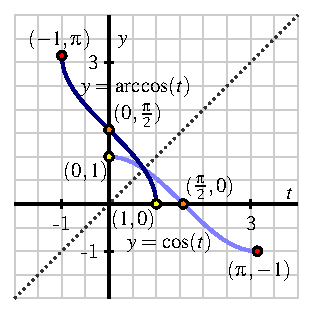
\includegraphics{inverse-trig-arccos-graph.pdf}
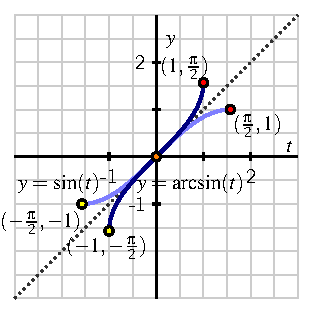
\includegraphics{inverse-trig-arcsin-graph.pdf}
\end{image}
\par
The domain of $y = f^{-1}(t) = \arcsin(t)$ is $[-1,1]$ with corresponding range $[-\frac{\pi}{2}, \frac{\pi}{2}]$, and the arcsine function is always increasing.  These facts correspond to the domain and range of the restricted sine function and the fact that the restricted sine function is increasing on $[-\frac{\pi}{2},\frac{\pi}{2}]$.%
\par
The domain of $y = f^{-1}(t) = \arctan(t)$ is the set of all real numbers with corresponding range $(-\frac{\pi}{2}, \frac{\pi}{2})$, and the arctangent function is always increasing.  These facts correspond to the domain and range of the restricted tangent function and the fact that the restricted tangent function is increasing on $(-\frac{\pi}{2},\frac{\pi}{2})$.%
\begin{image}
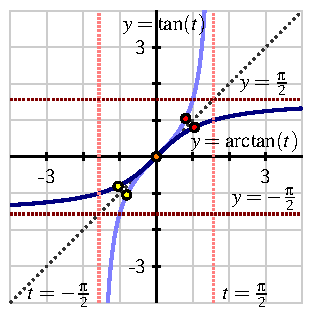
\includegraphics{inverse-trig-arctan-graph.pdf}
\end{image}
  \end{itemize}
\end{summary}


\end{document}
